\documentclass[letterpaper,11pt]{article}
\oddsidemargin -1.0cm \textwidth 17.5cm

\usepackage[utf8]{inputenc}
\usepackage[activeacute,spanish, es-lcroman]{babel}
\decimalpoint
\usepackage{amsfonts,setspace}
\usepackage{amsmath}
\usepackage{amssymb, amsmath, amsthm}
\usepackage{comment}
\usepackage{float}
\usepackage{amssymb}
\usepackage{dsfont}
\usepackage{anysize}
\usepackage{multicol}
\usepackage{enumerate}
\usepackage{graphicx}
\usepackage[left=1.5cm,top=2cm,right=1.5cm, bottom=1.7cm]{geometry}
\setlength\headheight{1.5em} 
\usepackage{fancyhdr}
\usepackage{multicol}
\usepackage{hyperref}
\usepackage{wrapfig}
\usepackage{subcaption}
\usepackage{siunitx}
\usepackage{cancel}
\usepackage{mdwlist}
\usepackage{svg}
\pagestyle{fancy}
\fancyhf{}
\renewcommand{\labelenumi}{\normalsize\bfseries P\arabic{enumi}.}
\renewcommand{\labelenumii}{\normalsize\bfseries (\alph{enumii})}
\renewcommand{\labelenumiii}{\normalsize\bfseries \roman{enumiii})}


\begin{document}

\fancyhead[L]{\itshape{Facultad de Ciencias F\'isicas y Matem\'aticas}}
\fancyhead[R]{\itshape{Universidad de Chile}}

\begin{minipage}{11.5cm}
    \begin{flushleft}
        \hspace*{-0.6cm}\textbf{FI1000-1 Introducción a la Física Clásica}\\
        \hspace*{-0.6cm}\textbf{Profesor:} Ignacio Bordeu\\
        \hspace*{-0.6cm}\textbf{Auxiliares:} Alejandro Cartes \& Simón Yáñez\\
        \hspace*{-0.6cm}\textbf{Ayudante:} Javier Cubillos\\
    \end{flushleft}
\end{minipage}

\begin{picture}(2,3)
    \put(366, 10){
\includegraphics[scale=0.9]{2020-1/Imágenes/logo/dfi-fcfm.pdf}}
\end{picture}

\begin{center}
	\LARGE\textbf{Trabajo Dirigido \#4}\\
	\Large{Preparación C3}
\end{center}

\vspace{-1cm}
\begin{enumerate}\setlength{\itemsep}{0.4cm}

\rfoot[]{pág. \thepage}

\item[]

% ---------------------------------------------------------
% ando sin inspiración :( no encontré más ejercicios buenos 
% 
% se repite el msje
% ---------------------------------------------------------

\item Dos objetos pueden deslizar sin roce por un riel circular de radio $R$ colocado en un plano vertical, como se muestra en la figura. El objeto de masa $3m$ se coloca en la parte más alta del riel y se conecta a un extremo de un resorte ideal de constante elástica $k$ y largo natural nulo. El otro extremo del resorte se fija a un punto colocado a una distancia $2R$ del centro del riel en el eje horizontal. El objeto de masa $m$ se coloca en reposo en la parte más baja del riel.

Al soltar el objeto de masa $3m$ del reposo, este se mueve por el riel para colisionar con el objeto de masa $m$, quedando adheridos. Calcule el valor de $m$ para que el par de objetos llegue justo hasta al punto $A$.

% \begin{figure}[htbp]
%   \centering
%   \svgpath{../../2023-1/img/TD 4}
%   \includesvg[width=0.7\textwidth]{P1.svg}
% \end{figure}

\item Una partícula de masa $m$, que se encuentra en una superficie inclinada, está atada al extremo de una cuerda de largo $L$, inicialmente en reposo y en una cierta posición caracterizada por el ángulo $\beta$ como se muestra la Figura 2. Considere que a partir de un ángulo $\theta$ la superficie un coeficiente de roce $\mu$ (tramo C-D en la Figura). Además, en el punto más bajo (B) hay un dispositivo que le entrega a la partícula $\Delta E$ de energía.

Determine el $\Delta E$ mínimo tal que la partícula logre llegar al punto más alto manteniendo la cuerda tensa.

\textbf{\textit{Hint}}: Haga un diagrama de cuerpo libre en la posición D. 

\begin{figure}[H]
        \centering
        \svgpath{../../2023-1/img/TD 4}
        \begin{subfigure}[t]{0.59\textwidth}
            \centering
            \includesvg[width=1\textwidth]{P1.svg}
            \caption{P1}
        \end{subfigure}
        \begin{subfigure}[t]{0.40\textwidth}
            \centering
            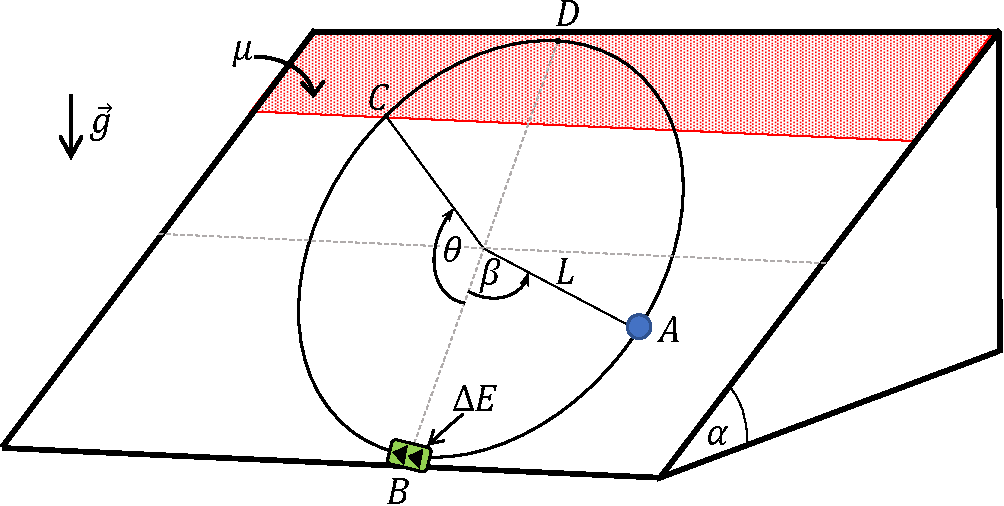
\includegraphics[width=1\linewidth]{2023-1/img/TD 4/p2c2.pdf}
            \caption{P2}
        \end{subfigure}
\end{figure}

\item Los tres carritos de la figura se encuentran sobre una superficie horizontal sin roce, solo la primera se mueve. $M$ y $2M$ chocan de forma perfectamente inelástica y esta luego choca elásticamente con $3M$.

\begin{multicols}{2}
    \begin{enumerate}
        \item Calcule la velocidad final de cada partícula.
        \item Calcule la pérdida de energía durante todo el proceso.
    \end{enumerate}
    
    \columnbreak
    
    \begin{figure}[H]
        \centering
        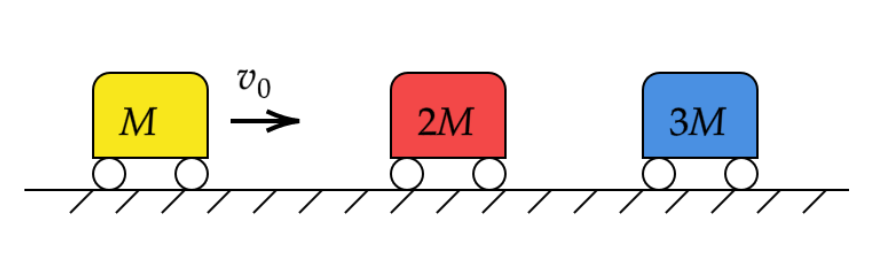
\includegraphics[width=0.4\textwidth]{2023-1/img/TD 4/P2 - TD 4.PNG}
    \end{figure}
\end{multicols}

\item Romeo y Julieta están sentados en un bote en reposo junto a un muelle. Julieta siente que está muy lejos de Romeo, por lo que decide ir a sentarse a su lado. Para ello camina a una rapidez constante $v$ relativa al agua.

Considere que la masa y la posición con respecto al muelle para Julieta, Romeo y el bote son ($m_j$, $x_j$), ($m_r$, $x_r$), ($m_b$, $x_b$) respectivamente. Además, considere que la distancia inicial que separa a Romeo y Julieta es inicialmente $x_j-x_r=D$.

\begin{multicols}{2}
    \begin{enumerate}
        \item Mientras Julieta está caminando, el bote y Romeo se mueven a rapidez $v'$ en dirección opuesta. Determine la razón $v'/v$
        
        \item Cuando Julieta finalmente se sienta junto a Romeo, ¿qué tan lejos se movió el bote con respecto al muelle?
    \end{enumerate}
    
    \columnbreak
    
    \begin{figure}[H]
        \centering
        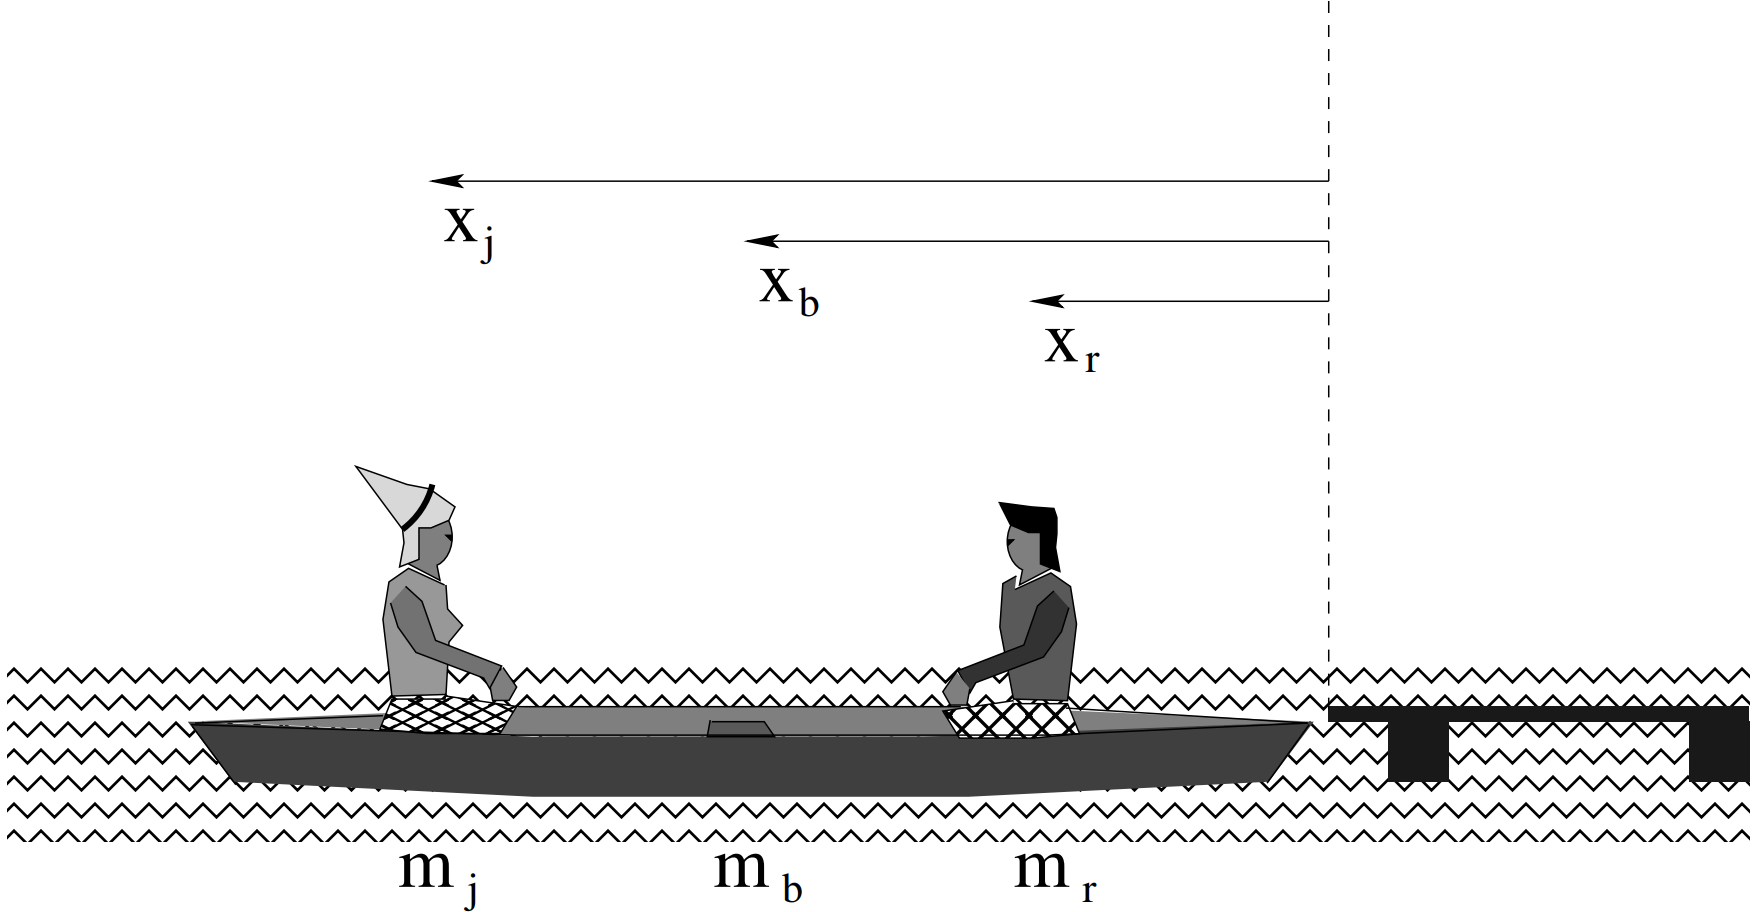
\includegraphics[width=0.7\linewidth]{2021-1/Imagenes/ejercicios/romeo-julieta.PNG}
        %\caption{Romeo y Julieta en el bote}
    \end{figure}

\end{multicols}
\textbf{\textit{Hint:}} Use centro de masa y conservación de momentum, desprecie el roce entre el agua y el bote


% Para imágenes vectoriales -> el texto tiene que estar en LaTeX
% \begin{figure}[htbp]
%   \centering
%   \svgpath{../Imagenes/ejercicios}  -> .. irse pa'trás 
%   \includesvg{ej5.svg}
% \end{figure}

\end{enumerate}
\end{document}